\documentclass[tikz,border=8pt]{standalone}
\usepackage{amsmath}
\usetikzlibrary{arrows.meta,positioning,fit,calc}

\begin{document}
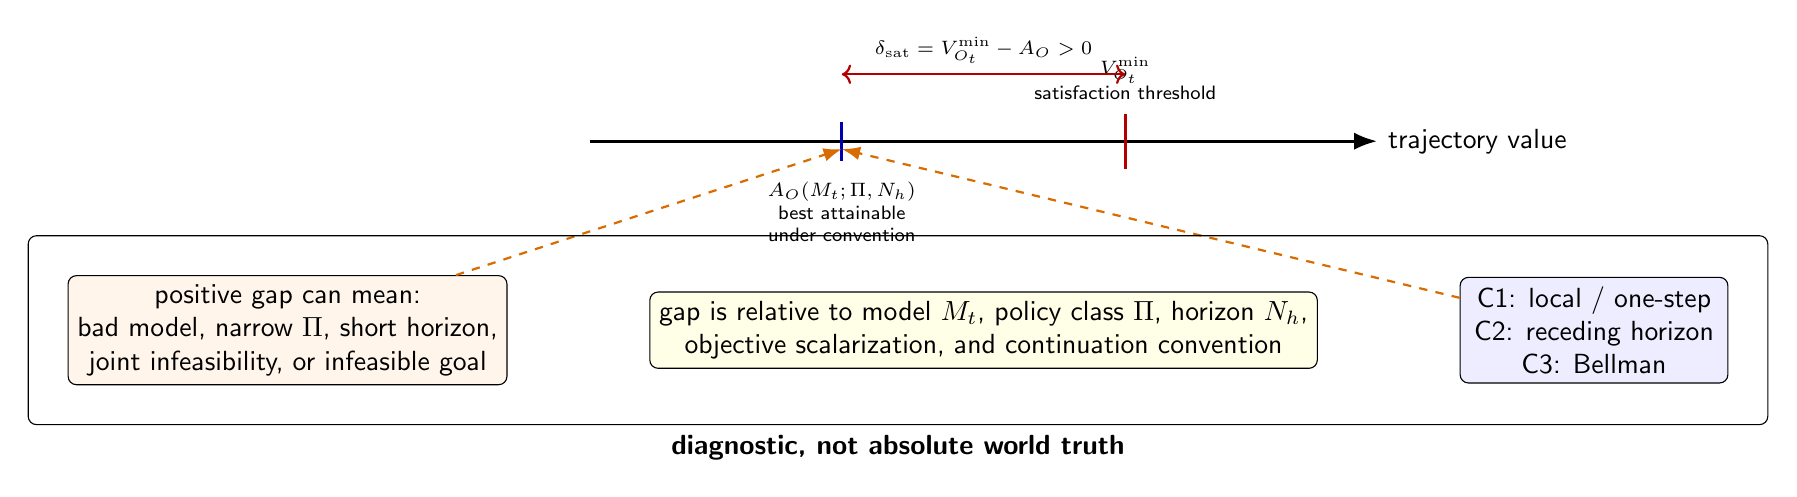
\begin{tikzpicture}[
  font=\sffamily,
  box/.style={draw, rounded corners=3pt, align=center, minimum width=34mm, minimum height=9mm, fill=white},
  note/.style={align=center, font=\sffamily\scriptsize},
  arrow/.style={-Latex, thick, draw=black!65},
  warn/.style={-Latex, thick, dashed, draw=orange!85!black}
]

\draw[-Latex, very thick] (0,0) -- (10,0) node[right] {trajectory value};
\draw[very thick, draw=blue!70!black] (3.2,-0.25) -- (3.2,0.25);
\node[note, below=4mm] at (3.2,0) {$A_O(M_t;\Pi,N_h)$\\best attainable\\under convention};
\draw[very thick, draw=red!70!black] (6.8,-0.35) -- (6.8,0.35);
\node[note, above=4mm] at (6.8,0) {$V_{O_t}^{\min}$\\satisfaction threshold};
\draw[<->, thick, draw=red!70!black] (3.2,0.85) -- node[above, note] {$\delta_{\rm sat}=V_{O_t}^{\min}-A_O>0$} (6.8,0.85);

\node[box, fill=yellow!10, minimum width=62mm] (relative) at (5,-2.4)
  {gap is relative to model $M_t$, policy class $\Pi$, horizon $N_h$,\\objective scalarization, and continuation convention};

\node[box, right=18mm of relative, fill=blue!7] (conv)
  {C1: local / one-step\\C2: receding horizon\\C3: Bellman};
\draw[warn] (conv) -- (3.2,-0.1);

\node[box, left=18mm of relative, fill=orange!8] (causes)
  {positive gap can mean:\\bad model, narrow $\Pi$, short horizon,\\joint infeasibility, or infeasible goal};
\draw[warn] (causes) -- (3.2,-0.1);

\node[draw, rounded corners=3pt, fit=(relative)(conv)(causes), inner sep=5mm,
  label={[font=\sffamily\bfseries]below:diagnostic, not absolute world truth}] {};

\end{tikzpicture}
\end{document}
